% ****** Start of file aipsamp.tex ******
%
%   This file is part of the AIP files in the AIP distribution for REVTeX 4.
%   Version 4.1 of REVTeX, October 2009
%
%   Copyright (c) 2009 American Institute of Physics.
%
%   See the AIP README file for restrictions and more information.
%
% TeX'ing this file requires that you have AMS-LaTeX 2.0 installed
% as well as the rest of the prerequisites for REVTeX 4.1
%
% It also requires running BibTeX. The commands are as follows:
%
%  1)  latex  aipsamp
%  2)  bibtex aipsamp
%  3)  latex  aipsamp
%  4)  latex  aipsamp
%
% Use this file as a source of example code for your aip document.
% Use the file aiptemplate.tex as a template for your document


\documentclass[%
 aip,12pt,
%jmp,%
%bmf,%
%sd,%
rsi,%
 amsmath,amssymb,
%preprint,%
 reprint,%
%author-year,%
%author-numerical,%
]{revtex4-1}

\usepackage{graphicx}% Include figure files
\usepackage{dcolumn}% Align table columns on decimal point
\usepackage{bm}% bold math
\usepackage{subcaption}


%\usepackage[mathlines]{lineno}% Enable numbering of text and display math
%\linenumbers\relax % Commence numbering lines
\newcommand{\refe}[1]{Eq. (\ref{#1})}


\begin{document}

% \preprint{AIP/123-QED}

\title[Replicating SINDy Results]{Replicating SINDy Results}
\large{

\author{Lia Gianfortone}
 % \altaffiliation[Also at ]{University of California, Santa Cruz}%Lines break automatically or can be forced with \\


\date{\today}% It is always \today, today,
             %  but any date may be explicitly specified

\begin{abstract}
System identification techniques that use sampled data to recover a system's governing equations are useful for a plethora of applications. The sparse identification of nonlinear dynamical systems algorithm (SINDy) relies on the assumption that the dynamics of many systems depend on only a few linear and nonlinear terms. This, paired with regression schemes, helps to guarantee a sparse solution for the set of coefficients of terms in the user-constructed function basis that SINDy outlines. This study analyzes the algorithm's performance in the recovery of several chaotic systems from noisy data.


\end{abstract}

\maketitle



\section{The SINDy Method\protect}
We consider systems of the form 
\begin{equation}
\frac{d}{dt}\bm{x}(t) = \bm{\dot{x}} = \bm{f}(\bm{x}(t))
\end{equation}
where $\bm{x}(t) \in \mathbb{R}^n$ is the state of the system at time $t$ and $\bm{f}$ consists of the governing equations of the system. 

Given $m$ (potentially noisy) measurements of the state $\bm{x}$ and its derivative $\bm{\dot{x}}$ over time, we arrange them into data matrices $\bm{X}$ and $\bm{\dot{X}}$ as follows
\begin{equation*}
  \bm{X} = \begin{bmatrix} 
        \bm{x}^T(t_1) \\ \bm{x}^T(t_2) \\ \vdots \\ \bm{x}^T(t_m)
      \end{bmatrix}
       = \begin{bmatrix}
          x_1(t_1) & x_2(t_1) & \cdots & x_n(t_1) \\
          x_1(t_2) & x_2(t_2) & \cdots & x_n(t_2) \\
          \vdots   & \vdots   & \ddots & \vdots   \\
          x_1(t_m) & x_2(t_m) & \cdots & x_n(t_m) 
        \end{bmatrix}
\end{equation*}

\begin{equation*}
  \bm{\dot{X}} = \begin{bmatrix} 
        \bm{\dot{x}}^T(t_1) \\ \bm{\dot{x}}^T(t_2) \\ \vdots \\ \bm{\dot{x}}^T(t_m)
      \end{bmatrix}
       = \begin{bmatrix}
          \dot{x}_1(t_1) & \dot{x}_2(t_1) & \cdots & \dot{x}_n(t_1) \\
          \dot{x}_1(t_2) & \dot{x}_2(t_2) & \cdots & \dot{x}_n(t_2) \\
          \vdots         & \vdots       & \ddots & \vdots  \\
          \dot{x}_1(t_m) & \dot{x}_2(t_m) & \cdots & \dot{x}_n(t_m)
        \end{bmatrix}.
\end{equation*}

To identify the active terms in the dynamics, we construct the system 
\begin{equation} \label{eqn:main}
  \bm{\dot{X}} = \bm{\Theta}(\bm{X})\bm{\Xi}
\end{equation}
where the state data are input to the library of linear and nonlinear candidate functions, $\bm{\Theta}(\bm{X})$, which consists of constant, polynomial, and trigonometric terms. The functions may be chosen based on hypotheses about the system dynamics based on symmetry, physics, measurement coordinates, or otherwise. The library of functions has the form
\begin{equation}
  \bm{\Theta}(\bm{X}) = 
  \begin{bmatrix}
    \mid & \mid   & \mid      &        & \mid       & \mid       &      \\
    1  & \bm{X}   & \bm{X}^{P_2}  & \cdots & \sin(\bm{X}) & \cos(\bm{X}) & \cdots \\
    \mid & \mid   & \mid      &        & \mid       & \mid       &
  \end{bmatrix}
\end{equation}
where polynomial cross-terms of degree $i$ are denoted $\bm{X}^{P_i}$. For example, $\bm{X}^{P_2}$ contains quadratic nonlinearities in the state $\bm{x}$,
\begin{equation*}
  \bm{X}^{P_2} = 
    \begin{bmatrix}
      x_1^2(t_1)  & x_1(t_1)x_2(t_1) & \cdots & x_2^2(t_1) & \cdots & x_n^2(t_1) \\
      x_1^2(t_2)  & x_1(t_2)x_2(t_2) & \cdots & x_2^2(t_2) & \cdots & x_n^2(t_2) \\
      \vdots    & \vdots         & \ddots & \vdots     & \ddots & \vdots   \\
      x_1^2(t_m)  & x_1(t_m)x_2(t_m) & \cdots & x_2^2(t_m) & \cdots & x_n^2(t_m) \\
    \end{bmatrix}.
\end{equation*}
The final term in \refe{eqn:main}, $\bm{\Xi} = [\bm{\xi}_1 \ \bm{\xi}_2 \cdots \bm{\xi}_n]$ is the desired sparse matrix of coefficients that identifies which of the candidate functions in $\bm{\Theta}(\bm{X})$ are active in the system. 

Solving for $\bm{\Xi}$ requires a distinct optimization of each column, corresponding to each of the $n$ vector equations that guide the system. This has the form
\begin{equation} \label{eqn:vector}
  \bm{\dot{x}} = \bm{f}(\bm{x}) = \bm{\Xi}^T(\bm{\Theta}(\bm{x}^T))^T.
\end{equation}
Algorithms to perform the desired sparse regression of \refe{eqn:vector} include the least absolute shrinkage and selection operator (LASSO) \cite{LASSO} that uses the $L_1$-norm to ensure sparsity and the sequential least-squares method. In this study, sequential least-squares was the method of choice.


\begin{figure*}[t]
\centering
\begin{subfigure}{.5\textwidth}
  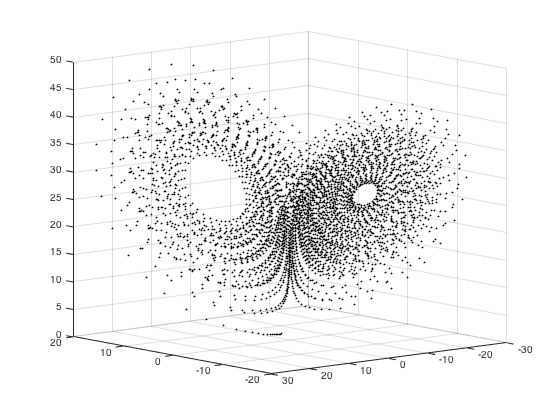
\includegraphics[width=.8\linewidth]{L_A.png}
\end{subfigure}%
\begin{subfigure}{.5\textwidth}
  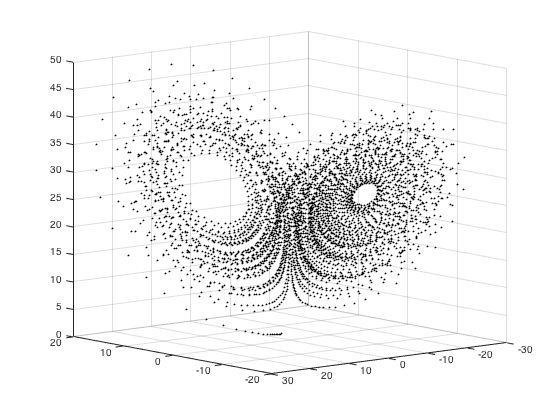
\includegraphics[width=.8\linewidth]{L_S.png}
\end{subfigure}
\caption{(Left) Known Lorenz solution for $\sigma=10, \ \beta=8/3, \ \rho=28$. (Right) Reconstruction of the system using SINDy solution with $\bm{\dot{X}}$ noise $\eta=0.2$ for a max coefficient error of 0.002. \label{fig:Lorenz}}
\end{figure*}


\subsection{Lorenz Attractor}
The Lorenz system is an interesting test for the SINDy method. The known dynamics are 
\begin{align}
  \dot{x} &= \sigma(y - x) \\
  \dot{y} &= x(\rho - z) - y \\
  \dot{z} &= xy - \beta z.
\end{align}
This system demonstrates chaotic behavior under certain conditions and is observably sparse in a Cartesian function space with only two nonlinear terms, $xz$ in $\dot{y}$ and $xy$ in $\dot{z}$. 

Data is generated in Matlab using the \verb|ode45| function and the chaotic parameters
\begin{equation}
  \sigma=10 \qquad \beta=8/3 \qquad \rho=28.
\end{equation} 
Random Gaussian noise is added to the $\bm{\dot{X}}$ data to challenge the algorithm. For noise amplitude $\eta=.3$ the maximum error between the known and discovered coefficients was .003. Noise amplitude $\eta=0.2$ resulted in a max error of .002 and for $\eta=0.1$ the max error significantly decreased to 0.0001. Figure \ref{fig:Lorenz} shows the solution generated by \verb|ode45| beside SINDy's interpretation of the system. The close agreement of the coefficients confirms the accuracy of SINDy's results but for chaotic systems such as those studied in this paper, even slight disturbances in trajectories will result in dramatically different systems and a later time. For this reason, when studying chaotic systems, we see that reducing the noise is critical to obtaining a well-resolved solution and measurements over a large span of time will increase the error of the identified solution based on the properties of chaotic systems alone. 





\section{SINDy for Discrete Systems}
The SINDy method can be adapted to determine the dynamics governing discrete systems as well. Discrete systems have the form 
\begin{equation} \label{discrete}
  \bm{x}_{k+1} = \bm{f}(\bm{x}_k)
\end{equation}
and are particularly well suited for the SINDy algorithm due to the absence of errors from the measurement or generation of state derivative data. The $m$ data points can be arranged into two matrices
\begin{equation}
  \bm{X}_1^{m-1} = 
    \begin{bmatrix}
      \bm{x}_1^T \\ \bm{x}_2^T \\ \vdots \\ \bm{x}_{m-1}^T
    \end{bmatrix} \ \ 
  \bm{X}_2^{m} = 
    \begin{bmatrix}
      \bm{x}_2^T \\ \bm{x}_3^T \\ \vdots \\ \bm{x}_{m}^T
    \end{bmatrix}.
\end{equation}
Identifying $\bm{f}(\bm{x}_k)$ in \refe{discrete} with SINDy consists of selecting a function basis $\bm{\Theta}(\bm{x}^T)$ and constructing the relation between each state and the one following it:
\begin{equation}
  \bm{X}_2^m = \bm{\Theta}(\bm{X}_1^{m-1})\bm{\Xi}
\end{equation}
so that 
\begin{equation}
  \bm{f}(\bm{x}_k) = \bm{\Xi}^T \bm{\Theta}(\bm{x}^T)^T.
\end{equation}
As before, the solution $\bm{\Xi}$  is obtained with column-by-column optimization.

\section{Duffing Map}


One discrete, nonlinear chaotic relation of interest is the Duffing map, a discrete for of the Duffing equation, to be discussed later,
\begin{align}
  x_{k+1} &= y_k \\ 
  y_{k+1} &= -\beta x_k + \alpha y_k - y_k^3.
\end{align}
Choosing $\alpha = 2.75$ and $\beta=0.2$ guarantees chaotic behavior in the system and our satisfaction in the problem as a test of SINDy for discrete systems. Figure \ref{fig:DD} shows the side-by-side analytical and SINDy results for the system. Due to the lack of error from the absent $\bm{\dot{X}}$ data, SINDy recovered the solution with machine precision accuracy.


\begin{figure*}[t]
\centering
\begin{subfigure}{.5\textwidth}
  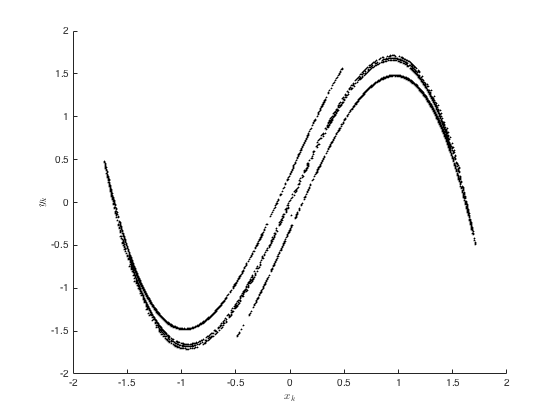
\includegraphics[width=.8\linewidth]{DD_A.png}
\end{subfigure}%
\begin{subfigure}{.5\textwidth}
  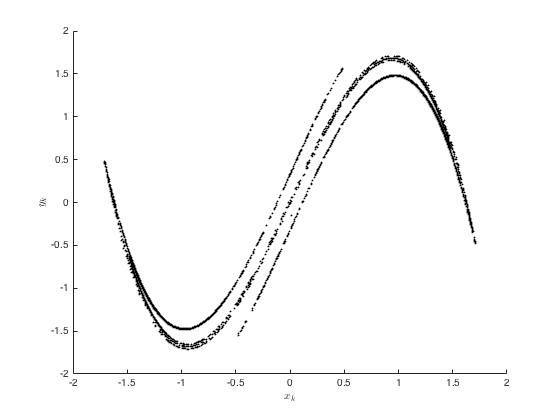
\includegraphics[width=.8\linewidth]{DD_S.png}
\end{subfigure}
\caption{Here is my caption\label{fig:DD}}
\end{figure*}


\section{SINDy for Systems with External Forcing\label{ext}}
Identifying the dynamics of systems with purely external forcing is a straightforward procedure if the control measurements are known. The control vectors are entered in a data matrix $\bm{Y}$ as
\begin{equation}
  \bm{Y} = 
    \begin{bmatrix}
      \bm{u}(t_1)^T \\ \bm{u}(t_2)^T \\ \vdots \\ \bm{u}(t_m)^T
    \end{bmatrix}
\end{equation}
and the selection of basis functions in $\bm{\Theta}$ is expanded to include control terms including cross-terms with the state variables. Optimization is then performed on the columns of 
\begin{equation} \label{control}
    \bm{\dot{X}} = \bm{\Theta}(\bm{X},\bm{Y})\bm{\Xi}
\end{equation}
to determine a sparse $\bm{\Xi}$ that identifies the dynamics of the system regardless of the control that is acting on it, so long as the control is itself not a function of the state.

\section{Duffing Equation}
The Duffing equation describes a second order nonlinear differential equation with external and sinusoidal forcing. The equation models damped and driven oscillators including the motion of a classical particle in a double well potential. The equation is
\begin{equation}
  \ddot x + \delta \dot x + \alpha x + \beta x^3 = \gamma \cos(\omega t).
\end{equation}
Systems governed by the Duffing equation will exhibit chaotic behavior for certain values of $\alpha,\ \beta,\ \gamma,$ and $\delta$.
Up until this point in the study, we have not considered using SINDy to determine coefficients in higher order differential equations that govern a measurable system. This is no obstacle as we recall that a $p$-th order differential equation can be separated in to $p$ first order differential equations. Thus the Duffing equation can be rewritten as 
\begin{align}
  \dot x &= v \\
  \dot v &= -\alpha x -\beta  x^3 - \delta v + \gamma \cos(\omega t)
\end{align}
and the dynamics can then be recovered with with regression on the relation
\begin{equation}
    \bm{[\dot{X}\ \dot{V}]} = \bm{\Theta}(\bm{[X\ V]},\bm{Y})\bm{\Xi}.
\end{equation}
The top row in figure \ref{fig:CD} shows the analytical and recovered dynamics for $\gamma = 8$ and the lower row shows the analytical solution and the constructed solution using the $\Xi$ solution obtained from the top row's computation but for $\gamma=10$. The computation that yielded the provided figures was done for $\bm{\dot{X}}$ noise with amplitude $\eta=.2$. This resulted in a maximum error between the known and discovered coefficients of .14. This is a substantial error that decreases to .0059 if the noise amplitude is $\eta=0.1$. This reinforces the previous deduction that low noise is critical for good system recovery.


\begin{figure*}[t]
\centering
\begin{subfigure}{.5\textwidth}
  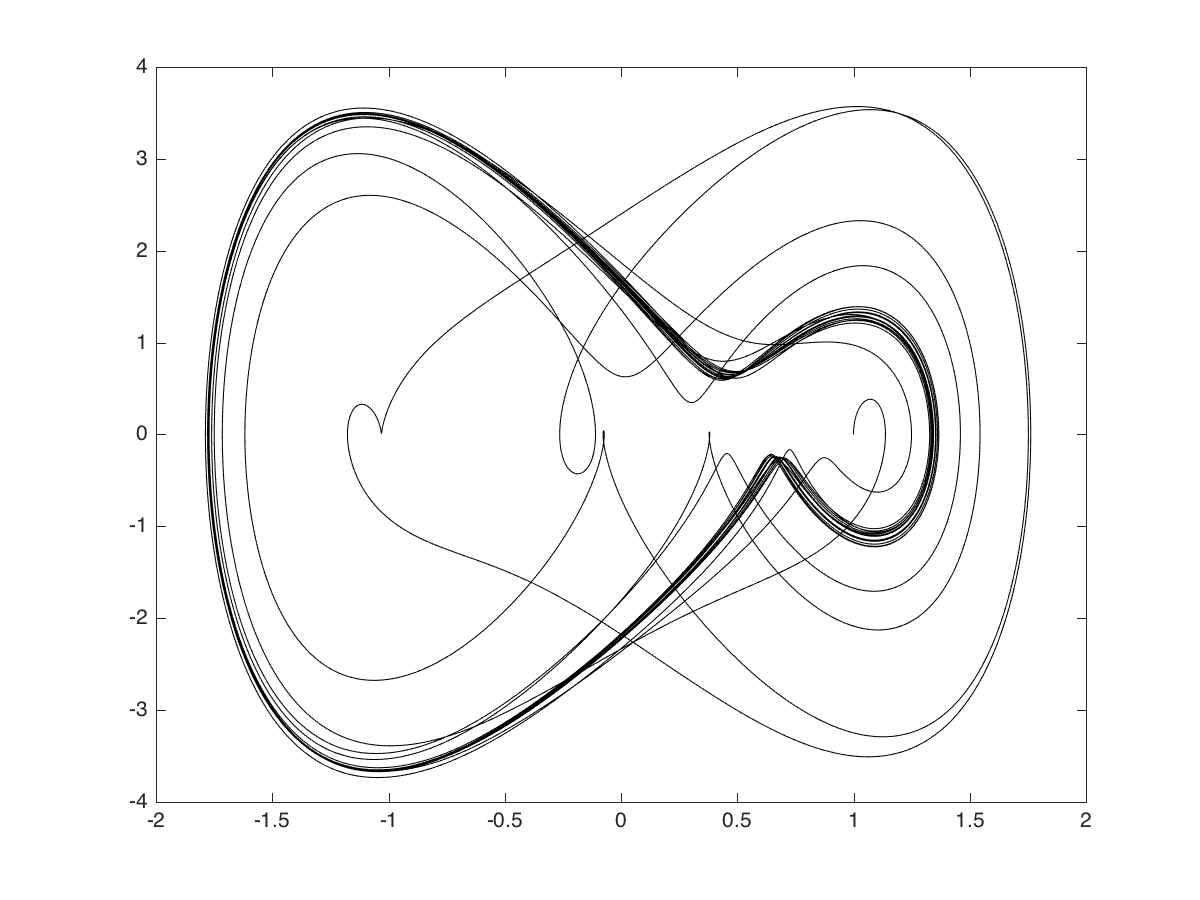
\includegraphics[width=.8\linewidth]{CD_A1.png}
\end{subfigure}%
\begin{subfigure}{.5\textwidth}
  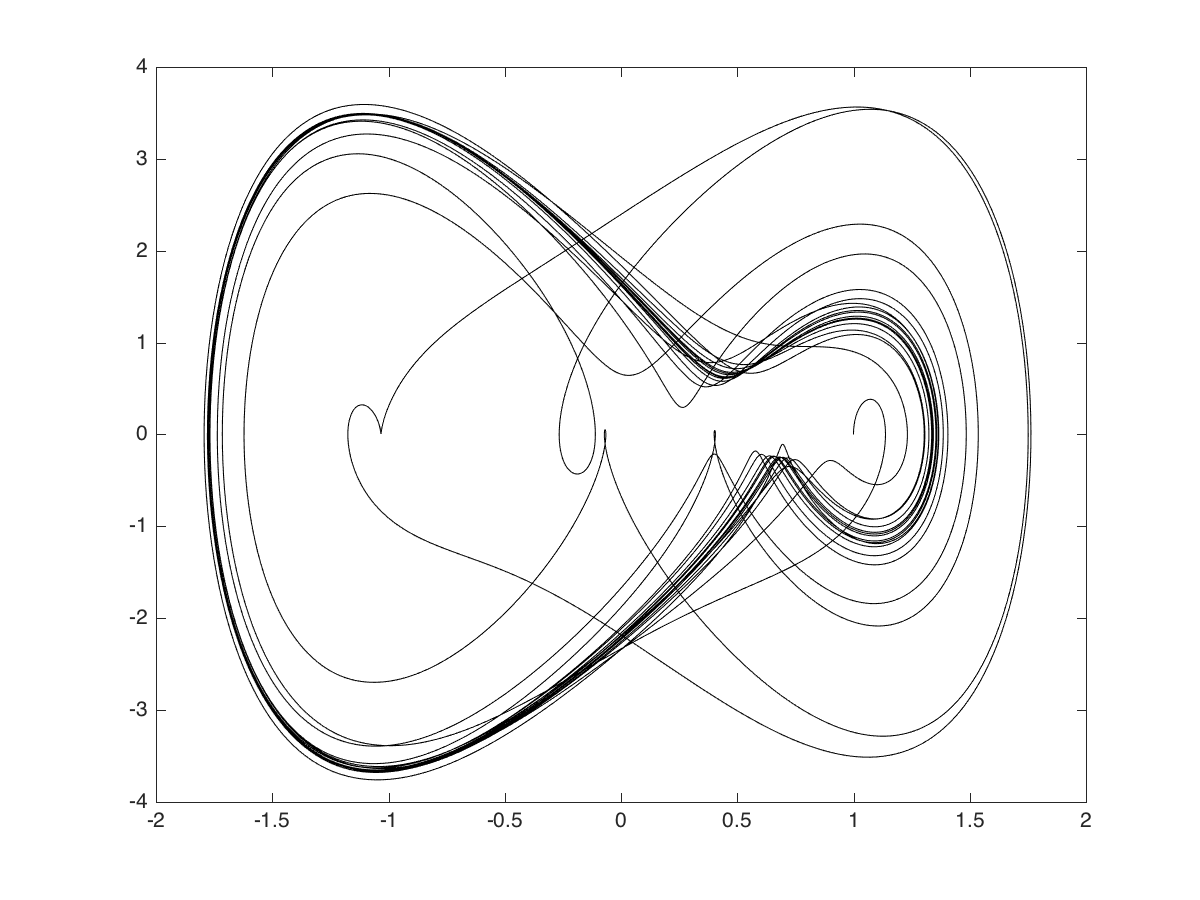
\includegraphics[width=.8\linewidth]{CD_S1.png}
\end{subfigure}
\begin{subfigure}{.5\textwidth}
  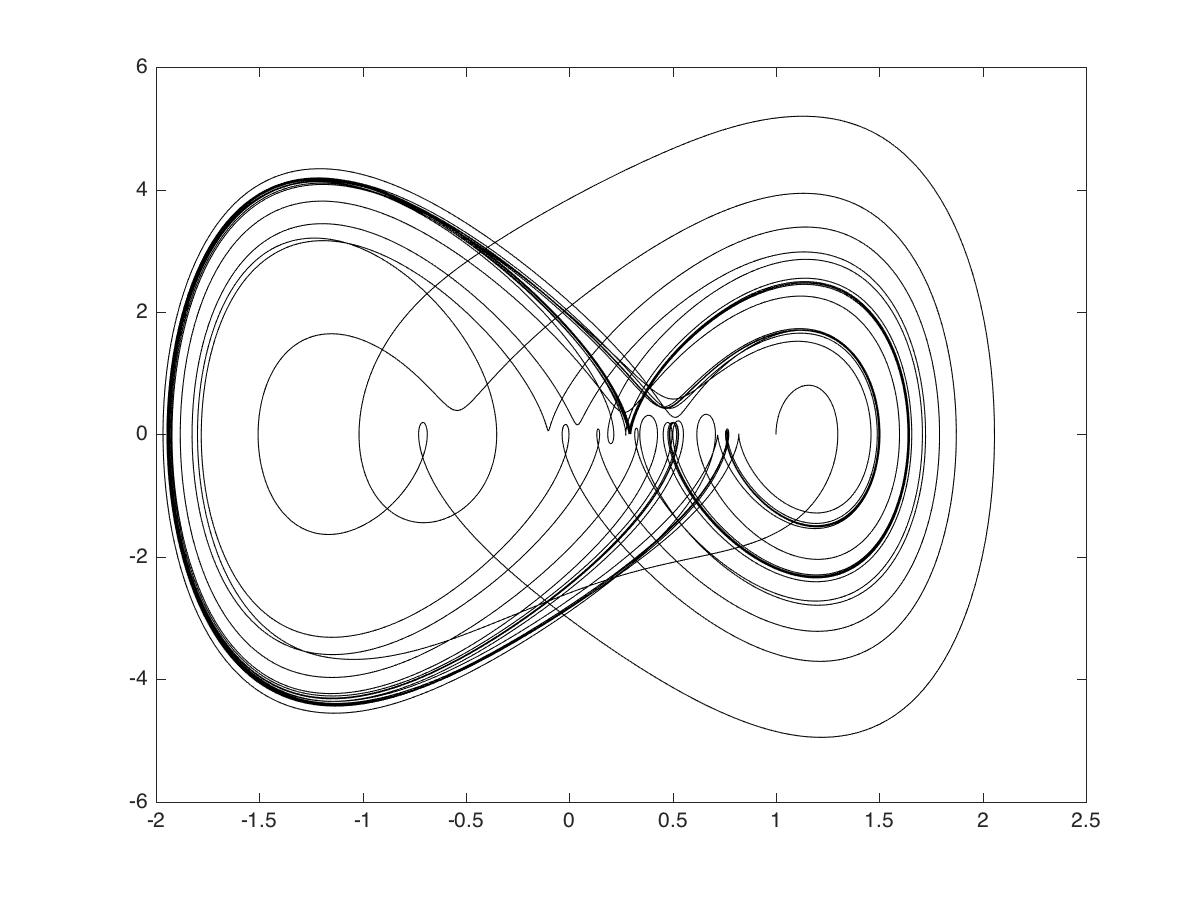
\includegraphics[width=.8\linewidth]{CD_A2.png}
\end{subfigure}%
\begin{subfigure}{.5\textwidth}
  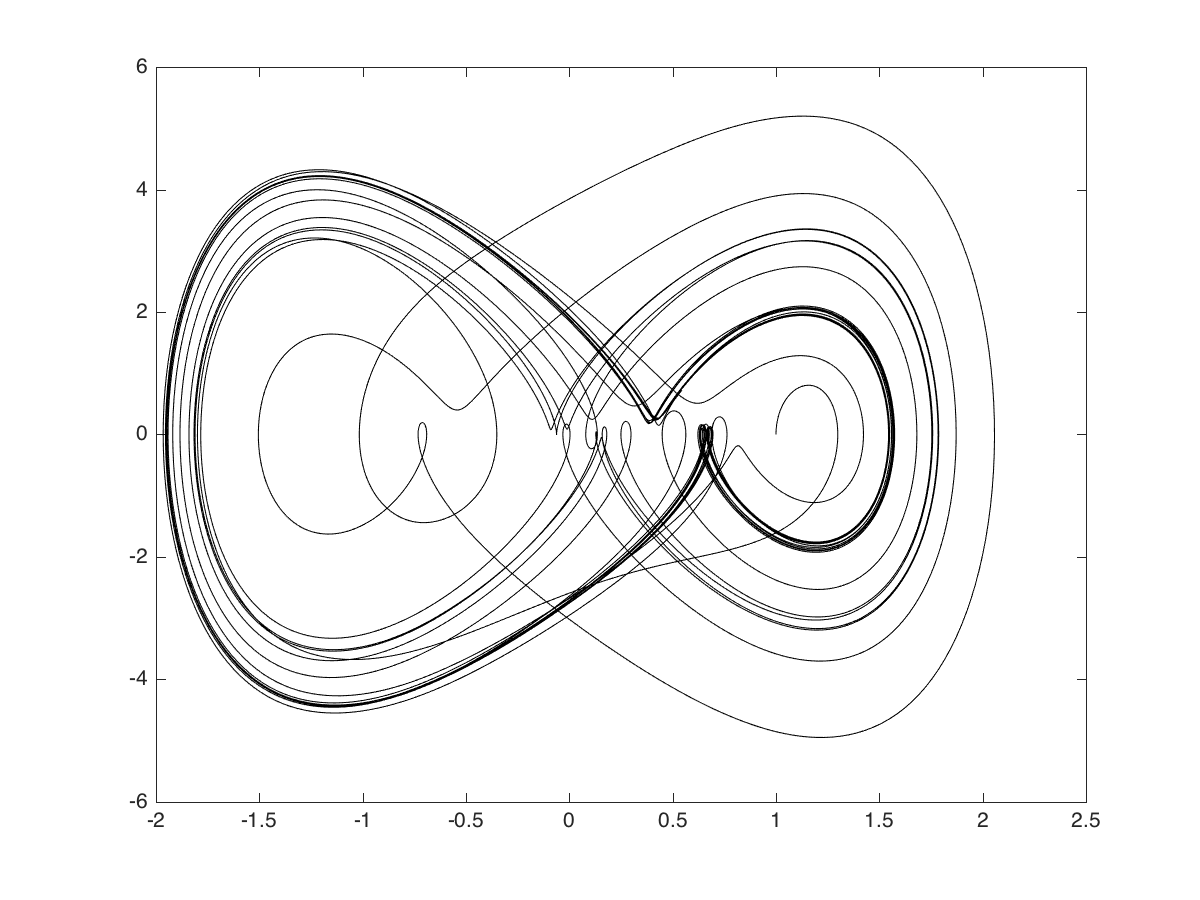
\includegraphics[width=.8\linewidth]{CD_S2.png}
\end{subfigure}
\caption{Here is my caption\label{fig:CD}}
\end{figure*}


\section{SINDYc Algorithm}
If forcing in a system includes feedback so that $\bm{u} = \bm{u}(\bm{x})$, the method described in Section \ref{ext} will be insufficient since \refe{control} will be ill-conditioned. A recent paper suggests first solving 
\begin{equation}
  \bm{Y} = \bm{\Theta}(\bm{X})\bm{\Xi}_u
\end{equation}
with a perturbed control signal, $\bm{u}$. Perturbations can be in the form of an impulse, a step, or white noise and will aid in differentiating the internal feedback from the inherent system dynamics when solving \refe{control}. The nuances of this adaptation of the method are not fully understood but would be an interesting continuation of this study. 


\section{Possible Problems}

Potential hangups in the implementation of this method may stem form poor choice of candidate functions or measurement coordinates, dynamics that are dependent on small coefficients, large noise in data, and overwhelming computational expense. Should any of the above occur, the simulation of the system using the state measurements and the solved-for coefficient matrix will not match the observed dynamics, indicating that further analysis or a reformatting of the problem is necessary.

\subsection{Bad Candidate Functions or Coordinates}
SINDy will produce poor solutions if the measurement coordinates or nonlinear function basis do not suit sparse representation, or if the function basis does not completely represent the possible dynamics of the system. Identifying and amending such an issue first consists of arbitrarily testing different function bases. If the inconsistency between the measured and simulated data persists, it may instead be due to feedback or excessive noise in the system.

\subsection{Small Dependence on Terms}
If using a regression algorithm such as sequential least-squares, the threshold for which terms are set to 0 to induce sparsity may be larger than the desired coefficients. This will again result in an incorrect simulation and could be resolved by lowering the threshold or rescaling the problem.

\subsection{Computational Expense}
Given that computation of $\bm{\Theta}(\bm{X})$ grows factorially with $n$, the dimension of the state, the SINDy method is less preferable than dynamic mode decomposition (DMD) which uses single value and eigen- decompositions to identify the normal modes of linear systems. Thus if a system is expected or known to be linear, the DMD method would be a better first choice of system identification. If the system is not linear, other dimensionality-reduction algorithms may prove useful in conjunction with SINDy.




\section{Conclusion}

Advances in this method might involve assimilation of dimensionality-reduction algorithms as aforementioned or an improved conveyance of the variation on the method to include feedback control. This recent algorithm holds promise of lending itself to a myriad of applications for which nonlinear dynamics are sought.


}


\nocite{*}
% {\footnotesize
\bibliography{Report}% Produces the bibliography via BibTeX.
% }

\end{document}
%
% ****** End of file aipsamp.tex ******